\documentclass[11pt,leqno]{beamer}
\usepackage{makecell}
\usepackage{ifxetex}
\usepackage{xcolor}
\ifxetex

  \usepackage[T1]{fontenc}
  \usepackage[no-math]{fontspec}

  \usefonttheme{serif}
  \setmainfont{Times NR MT Std}
H
  \usepackage[cal=euler, calscaled=1.0,
	      scr=boondox, scrscaled=1.0]{mathalfa}

  \let\hbar\relax
  \usepackage[noamssymbols,mtpcal,mtphrb,mtpfrak,
  	      subscriptcorrection,zswash]{mtpro2}
\else
  %\usepackage{lmodern}
  %\usepackage{mathrsfs}
  \usefonttheme{professionalfonts}
  \usepackage{stix}
  \newcommand{\mbf}{\mathbf} % to match mt2pro
\fi

\usetheme{metropolis}
\usepackage{appendixnumberbeamer}

%\usepackage{booktabs}
%\usepackage[scale=2]{ccicons}

%\usepackage{pgfplots}
%\usepgfplotslibrary{dateplot}

%\usepackage{xspace}
%\newcommand{\themename}{\textbf{\textsc{metropolis}}\xspace}

%\setbeamertemplate{bibliography item}{}


% BASIC PACKAGES %

\usepackage{makecell}
\usepackage{graphicx}
\usepackage{enumitem}
\usepackage{booktabs}
\usepackage{framed}
\usepackage{multirow}
\usepackage{scrextend}
\usepackage{stackengine}
\usepackage{subcaption}
\usepackage{comment}
\usepackage{url}
\usepackage{bm}
\usepackage[bottom]{footmisc}

% MARGIN NOTES %

\usepackage{marginnote}
\usepackage{setspace}

\newcommand{\lmn}[1]{{\reversemarginpar \setstretch{0.64} %
	\marginnote{{\scriptsize \bambootext{\emph{#1}}}}} }

\newcommand{\rmn}[1]{{\normalmarginpar \setstretch{0.64} %
	\marginnote{{\scriptsize \bambootext{\emph{#1}}}}} }

\setlength\marginparwidth{64pt}

% RAISE/LOWER %

\makeatletter
\newcommand{\raisemath}[1]{\mathpalette{\raisem@th{#1}}}
\newcommand{\raisem@th}[3]{\raisebox{#1}{$#2#3$}}
\makeatother

% HIDE MACRO %

\newif\ifhide
\hidetrue %\hidefalse
\newcommand{\hide}[1]{\ifhide {} \else {#1} \fi} 

% EMPHASIZE BOX %

\usepackage{empheq}
\newcommand{\widefbox}[1]{\fbox{\hspace{0.33in}#1\hspace{0.33in}}}


% CHAR MAPS: e.g. \calS for \mathcal{S}  %

\usepackage{pgffor}

\foreach \x in {A,...,Z}{%
  \expandafter\xdef\csname cal\x\endcsname{\noexpand %
	\ensuremath{\noexpand\mathcal{\x}}}
  \expandafter\xdef\csname scr\x\endcsname{\noexpand %
	\ensuremath{\noexpand\mathscr{\x}}}
  \expandafter\xdef\csname bb\x\endcsname{\noexpand %
	\ensuremath{\noexpand\mathbb{\x}}}
  \expandafter\xdef\csname rm\x\endcsname{\noexpand %
	\ensuremath{\noexpand\mathrm{\x}}}
  \expandafter\xdef\csname bf\x\endcsname{\noexpand %
	\ensuremath{\noexpand\mathbf{\x}}}
}

% ACCENTS %

\newcommand{\wh}[1]{\widehat{#1}}
\newcommand{\wt}[1]{\widetilde{#1}}

% SPACING %
\newcommand{\hs}[1]{ \hspace{#1pt} }

\newcommand{\mptt}{\hspace{-2pt}  }
\newcommand{\mpt}{ \hspace{-1pt}  }
\newcommand{\mhpt}{\hspace{-0.5pt}}
\newcommand{\hpt}{ \hspace{0.5pt} }

\newcommand{\pt}{ \hspace{1pt}  }
\newcommand{\ptt}{ \hspace{2pt} }
\newcommand{\pttt}{ \hspace{3pt}}
\newcommand{\ptttt}{\hspace{4pt}}

% BASIC MATH %

%\newcommand{\bst}{ \hspace{1.5pt} | \hspace{1.5pt} }
%\newcommand{\cst}{ \hspace{0.5pt} : \hspace{0.5pt} }
%\newcommand{\sst}{ \hspace{2pt} ; \hspace{0.5pt} }
\newcommand{\evl}{ \left| \right. }

\newcommand{\abs}[1]{\left| {#1} \right|}
\newcommand{\ceil}[1]{\left\lceil #1 \right\rceil}
\newcommand{\floor}[1]{\left\lfloor #1 \right\rfloor}

% ARROWS %

%\newcommand{\upto}{ \uparrow }
%\newcommand{\downto}{ \downarrow }
%\newcommand{\nto}{ \nrightarrow }

% TEXT %

%\newcommand{\tq}[1]{{\textquotedblleft #1\textquotedblright}}
%\newcommand{\ts}[2]{{#1\textsubscript{#2}}}


% Brackets, Parentheses, etc %

\newcommand{\pa}[1]{\hspace{1pt} \left( \hspace{0.5pt} %
	{#1} \hspace{0.5pt} \right) \hspace{1pt}}
\newcommand{\qa}[1]{\hspace{1pt} \left[ \hspace{0.5pt} %
	{#1} \hspace{0.5pt} \right] \hspace{1pt}}
\newcommand{\fa}[1]{\hspace{1pt} \left \{ \hspace{0.5pt} % 
	{#1} \hspace{0.5pt} \right \}\hspace{1pt}}
\newcommand{\za}[1]{\hspace{1pt} \left\langle \hspace{0.5pt} %
	{#1} \hspace{0.5pt} \right\rangle \hspace{1pt}}

\newcommand{\p}[1]{ \hspace{1pt} ( \hspace{0.25pt} %
	{#1} \hspace{0.25pt} ) \hspace{1pt}}
\newcommand{\q}[1]{ \hspace{1pt} [ \hspace{0.25pt} %
	{#1} \hspace{0.25pt} ] \hspace{1pt}}
\newcommand{\f}[1]{ \hspace{1pt} \{ \hspace{0.25pt} %
	{#1} \hspace{0.25pt} \} \hspace{1pt}}
\newcommand{\z}[1]{ \hspace{1pt} \langle \hspace{0.25pt} %
	{#1} \hspace{0.25pt}\rangle\hspace{1pt}}
\newcommand{\g}[1]{ \hspace{1pt} \langle \hspace{0.25pt} %
	{#1} \hspace{0.25pt}\rangle\hspace{1pt}}

\newcommand{\pp}[1]{ \hspace{1pt} \big( \hspace{0.5pt} %
	{#1} \hspace{0.5pt} \big) \hspace{1pt}}
\newcommand{\qq}[1]{ \hspace{1pt} \big[ \hspace{0.5pt} %
	{#1} \hspace{0.5pt} \big] \hspace{1pt}}
\newcommand{\ff}[1]{ \hspace{1pt} \big\{ \hspace{0.5pt} %
	{#1} \hspace{0.5pt} \big\} \hspace{1pt}}
\newcommand{\zz}[1]{ \hspace{1pt} \big\langle \hspace{0.5pt} %
	{#1} \hspace{0.5pt} \big\rangle \hspace{1pt}}

\newcommand{\ppp}[1]{ \hspace{1pt} \Big( \hspace{0.5pt} %
	{#1} \hspace{0.5pt} \Big) \hspace{1pt}}
\newcommand{\qqq}[1]{ \hspace{1pt} \Big[ \hspace{0.5pt} %
	{#1}  \hspace{0.5pt} \Big] \hspace{1pt}}
\newcommand{\fff}[1]{ \hspace{1pt} \Big\{ \hspace{0.5pt} %
	{#1}  \hspace{0.5pt} \Big\} \hspace{1pt}}
\newcommand{\zzz}[1]{ \hspace{1pt} \Big\langle \hspace{0.5pt} %
	{#1} \hspace{0.5pt} \Big\rangle \hspace{1pt}}

\newcommand{\pppp}[1]{ \hspace{1pt} \bigg(% 
	\hspace{0.5pt} {#1} \hspace{0.5pt} \bigg) \hspace{1pt}}
\newcommand{\qqqq}[1]{ \hspace{1pt} \bigg[% 
	\hspace{0.5pt} {#1} \hspace{0.5pt} \bigg] \hspace{1pt}}
\newcommand{\ffff}[1]{ \hspace{1pt} \bigg\{% 
	\hspace{0.5pt} {#1} \hspace{0.5pt} \bigg\} \hspace{1pt}}
\newcommand{\zzzz}[1]{ \hspace{1pt} \bigg\langle 
	\hspace{0.5pt} {#1} \hspace{0.5pt} \bigg\rangle \hspace{1pt}}


% REFERENCES & LABELS %

\makeatletter
\@ifpackageloaded{harvard}{}
  {\newcommand{\citeasnoun}{\cite}}
\makeatother

\newcommand{\ci}{\citeasnoun}
\newcommand{\cic}[2]{\citeasnoun[#1]{#2}}

\newcommand{\hci}[2]{ \href{#2}{\ci{#1}} }
\newcommand{\hcic}[3]{ \href{#3}{\cic{#1}{#2}} }
\newcommand{\hcite}[2]{ \href{#2}{\cite{#1}} }

\newcommand{\req}[1]{(\ref{#1})}






% PROBABILITY %

\newcommand{\cid}{\overset{\scrD}{\rightarrow}}
\newcommand{\eqd}{\overset{\scrD}{=}}
\newcommand{\cip}{\overset{p}{\rightarrow}}
\newcommand{\cas}{\overset{a.s.}{\rightarrow}}

\newcommand{\inds}[1]{ \mathbold{1}_{ \hspace{-1pt} {#1} }}
\newcommand{\indf}[1]{ \mathbold{1}_{ \hspace{-1pt} \f{ {#1} } }}
\newcommand{\var}{ \text{var} }
\newcommand{\cov}{ \text{cov} }

\newcommand{\Var}{ \mbf{Var}  }
\newcommand{\Cov}{ \mbf{Cov}  }
\newcommand{\Exp}{ \mbf{E}  }
\newcommand{\Prb}{ \mbf{P}  }
\newcommand{\Qrb}{ \mbf{Q} }

\newcommand{\re}{ \calE_a }

\renewcommand{\Re}{\mathfrak{R}}
\renewcommand{\Im}{\mathfrak{I}}


\newcommand{\rcll}{c{\`a}dl{\`a}g}


\newcommand{\blam}{ \bm{\Lambda} }




% Bamboo pallete %

\definecolor{deluge}{RGB}{124, 113, 173}
\definecolor{bamboo}{RGB}{220, 92, 5}
\definecolor{yellow}{RGB}{255, 172, 0}
\definecolor{orange}{RGB}{255, 144, 0}
\definecolor{oyster}{RGB}{151, 139, 125}
\definecolor{coral}{RGB}{199, 186, 167}
\definecolor{downy}{RGB}{110, 197, 184}
\definecolor{blueberry}{HTML}{6B7A8F}
\definecolor{alexbcolor}{HTML}{6088C7}

\def\delugetext#1{{\color{deluge}{{#1}}\color{deluge}}}
\def\bambootext#1{{\color{bamboo}{{#1}}\color{bamboo}}}
\def\yellowtext#1{{\color{yellow}{{#1}}\color{yellow}}}
\def\orangetext#1{{\color{orange}{{#1}}\color{orange}}}
\def\oystertext#1{{\color{oyster}{{#1}}\color{oyster}}}
\def\coraltext#1{{\color{coral}{{#1}}\color{coral}}}
\def\downytext#1{{\color{downy}{{#1}}\color{downy}}}



\setbeamercolor{frametitle}{bg=coral}
\setbeamercolor{progress bar}{fg=bamboo, bg=oyster}
\setbeamercolor{alerted text}{fg=bamboo}



\title{Explicit Solution for Position Constrained 
Minimum Variance Portfolios}
\date{Seminar at University of California, Berkeley\\March 3, 2020}
\author{Alex Bernstein\\
\url{abernstein@ucsb.edu}\\
joint work with Alexander Shkolnik \\ 
}
\institute{
{\it Department of Statistics \& Applied Probability } \\
University of California, Santa Barbara
% \titlegraphic{\hfill\includegraphics[height=1.5cm]{logo.pdf}}
} 

\begin{document}


\ifxetex
  \let\lsum\sum
  \renewcommand{\sum}{\bm{\lsum}}

  \let\lprod\prod
  \renewcommand{\prod}{\bm{\lprod}}
\else
\fi




\begin{frame}
\maketitle
\end{frame}

\newcommand{\af}{Y}
\newcommand{\df}{X}
\begin{frame}{The Minimum Variance Portfolio}
The Minimum Variance Portfolio  solves:
\begin{equation}
\begin{aligned}
 &\min_{x \in \bbr^p} x^\top \Gs x \\
  &\text{ subject to:} \\
  &\hspace{0.08in}\left\{
	\begin{array}{r}
	 \textstyle\sum\nolimits_k \hpt x_k =1 , \\
	\end{array} 
\right. \label{con}
\end{aligned}
\end{equation}
$\Gs$ is the covariance matrix for the vector of securities $x$.
Explicit Solution:
\begin{equation}
x = \frac{\Gs^{-1}\be}{\be^\T \Gs^{-1}\be}
\end{equation}

Each $x_i$ represents a ``proportion'' of the total investable assets.  Goal is to minimize ``risk''; in this case, risk is Variance.  

\end{frame}


\section{Context and History}
\begin{frame}{Why Minimum Variance Portfolio?}
Percent Return Over Time of Market vs. Minimum Variance Portfolio  for 1000 Largest US Stocks 
\begin{centering}
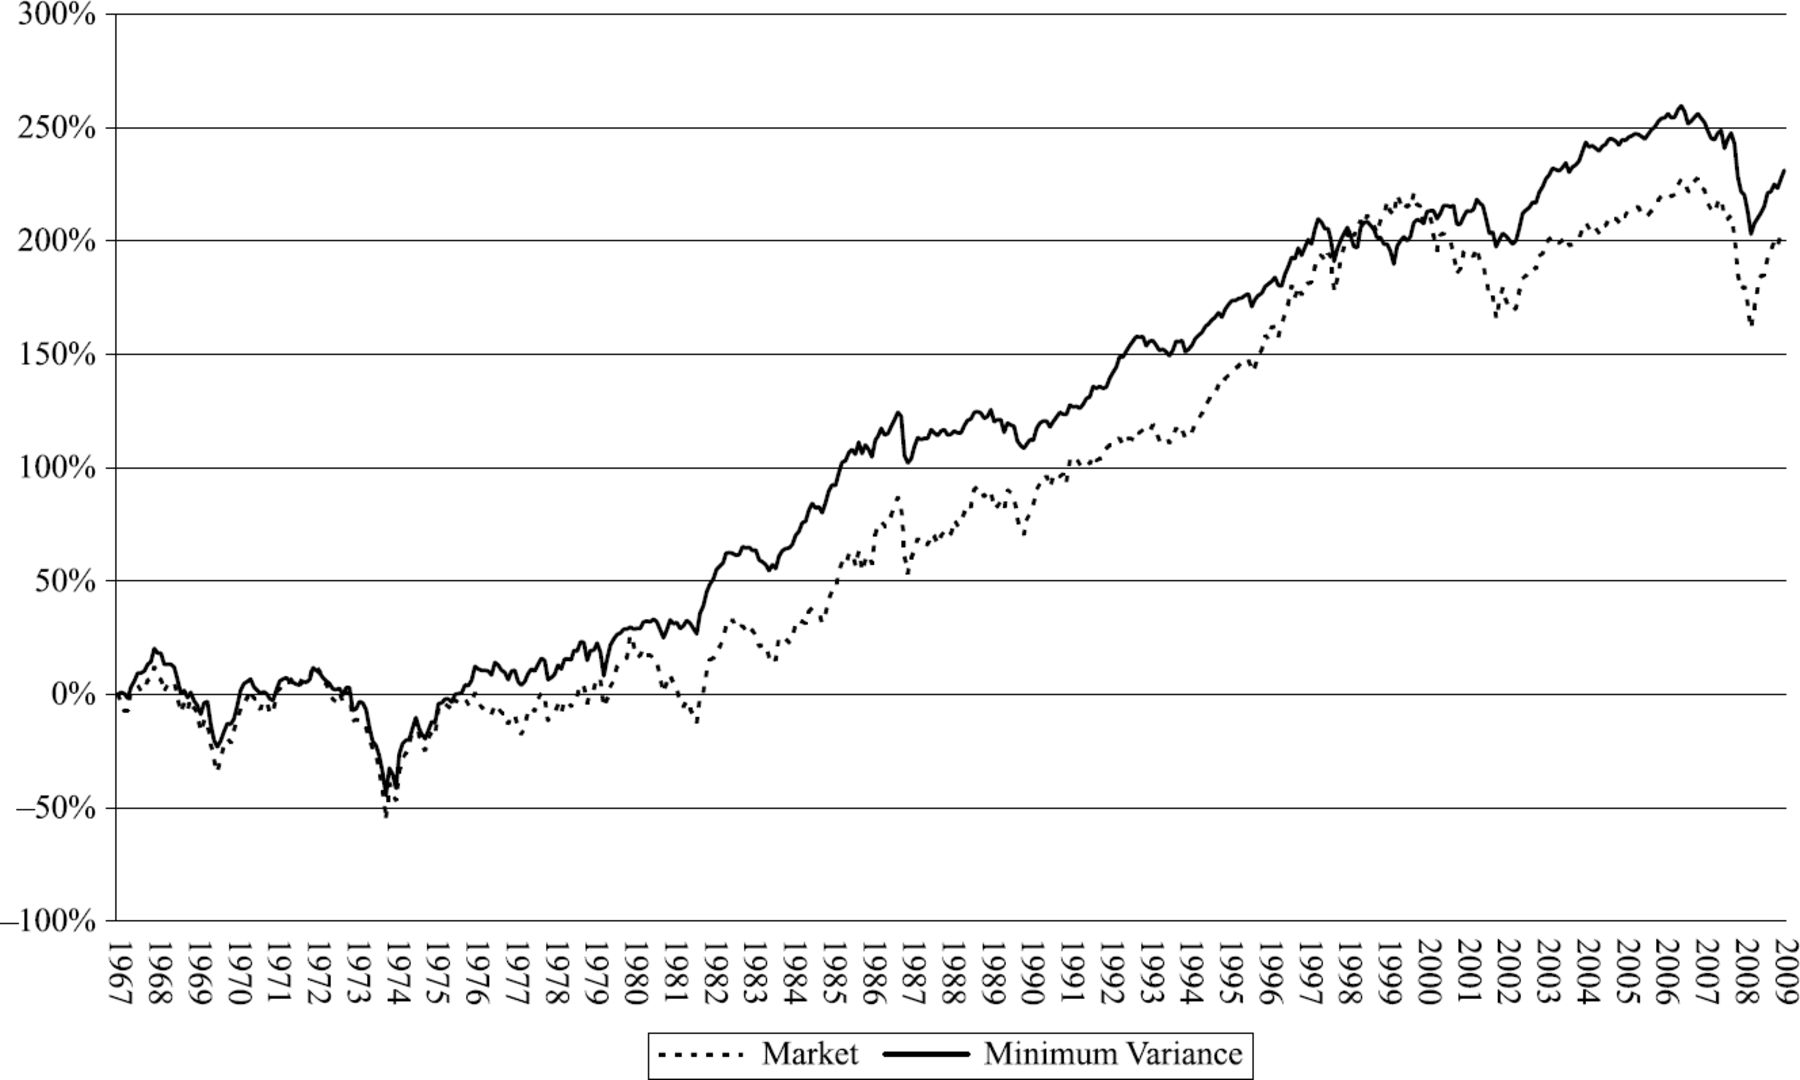
\includegraphics[scale=0.5]{CDPic.jpg}\\
\cite{c31}
\end{centering}\\
\begin{itemize}
\item Minimum Variance Portfolio has usually beaten Market Portfolio (1000 largest US Equities).  This is the Low-Volatility anomaly: low beta stocks get a higher than expected return.
\end{itemize}
\end{frame}

\begin{frame}{Why Long Only Constraints?}
\begin{itemize}
\item Markowitz actually included long-only constraints in his original paper; these were subsequently dropped from most formulations.
\item``imposing the no-short-sales constraints can help even when the constraints do not hold in the population.'' \cite{jnma}
\item No-Shortselling Constraints acts like a shrinkage estimator that prevents massive weights, i.e. exchanging a little bias for a reduction in variance.
\end{itemize}

\end{frame}

\begin{frame}{Portfolio Theory Origins of Quadratic Programming}
\begin{itemize}
\item Mean-Variance gives an early example of an algorithm to solve Quadratic Programs- the Critical Line Algorithm.
\item Other Algorithms  supplanted it; Markowitz was more focused on portfolio theory than mathematical optimization
\item Now we have robust and efficient numerical solvers for many real-world quadratic programs
\end{itemize}
\end{frame}





\section{Theorem}

\begin{frame}{Structural Model}
Structured Covariance matrix $\mat{\Gs}$ with $q$ factors:
\begin{equation}
\mat{\Gs} = \bB\bV \bB^\T + \Gd
\end{equation}
\[\bB = \underbrace{\begin{bmatrix}
 \vdots & \vdots & & \vdots\\
 \gb_1 & \gb_2 & \ldots & \gb_{q} \\
  \vdots & \vdots & & \vdots
\end{bmatrix}}_{p \times q}, \quad \Gd = \underbrace{\begin{bmatrix}
\gd_1^2 & & \\
& \ddots & \\
& & \gd_p^2
\end{bmatrix}}_{ p \times p}, 
\quad \bV = \underbrace{\begin{bmatrix}
\gs_1^2 & & \\
& \ddots & \\
& & \gs_q^2
\end{bmatrix}}_{ q \times q}
\]
Model assumes $q << p$. \\
\begin{itemize}
\item Interested in solutions with more factors
\item Want to analyze the underlying mathematics of minimum variance factor models
\end{itemize}
\end{frame}


\begin{frame}{Solution to the Unrestricted Markowitz Model}
Recall the solution minimum variance portfolio \textit{without} Long-Only Constraints:
\begin{equation}
x \propto w = \Gs^{-1} \be
\end{equation}
When $\Gs$ is a structural factor-model, we can write
\begin{equation}
w = \Gd^{-1}\paren{\be - \bB \gc}
\end{equation}
where $\gc \in \bbr^q$ solves:
\begin{equation} \label{theta_ls}
\paren{\mat{I} + \bV \bB^\T \Gd^{-1} \bB} \gc = \bV \bB^\T \Gd^{-1} \be
\end{equation}
\end{frame}




\begin{frame}{Main Theorem}
Let $\bB \in \bbr^{p\times q}$, $\bdel \in \bbr^{p \times p}_+$,  $\bV \in \bbr^{q \times q}_+$. Without loss of generality, assume $\Gd^{-1}\bB^\T \be\geq 0$ in each element. 
\begin{equation}
\begin{aligned}
 &\min_{x \in \bbr^p} x^\top (\bB \bV \bB^\T  + \Gd)x\\
  &\text{ subject to:} \\
  &\hspace{0.08in}\left\{
	\begin{array}{r}
	 \textstyle\sum\nolimits_k \hpt x_k =1 , \\
	 x_i \geq 0
	\end{array} 
\right. \label{con}
\end{aligned}
\end{equation}

\end{frame}

\begin{frame}{Main Theorem}
\begin{theorem}

There exists a unique minimizer to Equation \req{con} given by
\begin{equation}
x = \frac{w}{w^\T \be}
\end{equation}
where 
\begin{equation}
w = \Gd^{-1}\paren{\be - \bB \theta}_+
\end{equation}
Define: $\psi: \bbr^q \to \bbr^q$:
\begin{equation} 
\psi(z)= \bV \bB^\T \Gd^{-1}(\mat{e} - \bB z)_+
\end{equation}
 $\theta$ is the unique fixed point of $\psi$, i.e. $\psi(\theta)=\theta$.
\end{theorem}
\end{frame}

\begin{frame}{Geometry of the Solution}
The solution to the unrestricted problem is proportional to:
\begin{equation}
\be - \bB \gc = \be - \theta_1 \gc_1- \theta_2 \gc_2 - \ldots -\theta_q \gc_q
\end{equation}
The solution to the restricted problem is proportional to:
\begin{equation}
\paren{\be - \bB \theta}_+ = \paren{\be - \theta_1 \gb_1- \theta_2 \gb_2 - \ldots -\theta_q \gb_q}_+
\end{equation}
``Close to'' orthogonal to $\be$, under some restrictions.
\end{frame}


\begin{frame}{Idea of proof}
\begin{itemize}
\item  Introduce a change of variables to guarantee positivity of $w$ as the vector of elements $w_i^2$.
\item Establish an equivalence between the KKT Conditions and the Fixed Point under a certain orientation of $\bB$.
\end{itemize}

\end{frame}
\begin{frame}{Portfolio is also a Fixed-Point}
\begin{corollary}
$w$ is a $\bbr^p$-fixed point as well.
\end{corollary}
The existence of a solution to the mapping $w \mapsto \Gd^{-1}\paren{\be - \bB \bV \bB^\T w}_+$ is a direct consequence of the existence and uniqueness of a fixed point $\psi(\theta)=\theta$.
\end{frame}

\begin{frame}{Comments}
\begin{itemize}
\item The Long-Only Portfolio seems to be very quickly computable via fixed-point iterations on a slightly modified system akin to the calculation of the unconstrained portfolio; however convergence is not guaranteed.
\item There are other ways to compute this minimum without using Fixed-Point iterations.
\end{itemize}

\end{frame}

\section{One-Factor Theorem Analysis}


\begin{frame}{One Factor Model with Long Only Constraints}
Let $\gb \in \bbr^p$, and $\gd^2, \gs^2 \in \bbr_+$.  Under a single covariance factor, our minimization problem now becomes:
\begin{equation}
\begin{aligned}
 &\min_{x \in \bbr^p} x^\top (\gs^2 \gb \gb^\T  + \gd^2)x\\
  &\text{ subject to:} \\
  &\hspace{0.08in}\left\{
	\begin{array}{r}
	 \textstyle\sum\nolimits_k \hpt x_k =1 , \\
	 x_i \geq 0
	\end{array} 
\right. \label{con1}
\end{aligned}
\end{equation}
\textit{Can generalize to $\gd_1^2, \ldots, \gd_p^2$, but more notation for little gain.}
Recall, the solution is given by:
\begin{equation}
x_i \propto w_i =\frac{(1-\theta \gb_i)_+}{\gd^2}
\end{equation}
\end{frame}


\begin{frame}{Prior Work on Long-Only Factor Models}
\begin{itemize}

\item 1-factor version  published in 2011, \textit{with some slight caveats} \cite{c31}
\item Explained why large-$\gb_i$ weights are truncated to $0$
\item Proof was ``semi-formal'' and difficult to follow.

\end{itemize}
\end{frame}

\begin{frame}{Clarke Formula}
\begin{itemize}
\item Solution involved computation Fixed Point $\eta = \psi_c(\eta)$ of the awkward function:
\begin{equation}
 \psi_{c}(z) = \frac{1/\gs^2 + \sum_{\{i: \gb_i<z\}} \gb_i^2/\gd^2 }{ \sum_{\{i: \gb_i<z\}} \gb_i/\gd^2 }
\end{equation}

\item Solutions may not exist: e.g. $\gb = [-2,-1,1]^\T$ and $\gs^2 = \gd^2 = 1$.
\item Instead, of a fixed point, may have $\psi_c(\eta) = -\eta$; alternatively, a fixed point for $-\gb$.
\end{itemize}
\end{frame}
\begin{frame}{Existence Counter-Example}
\begin{centering}
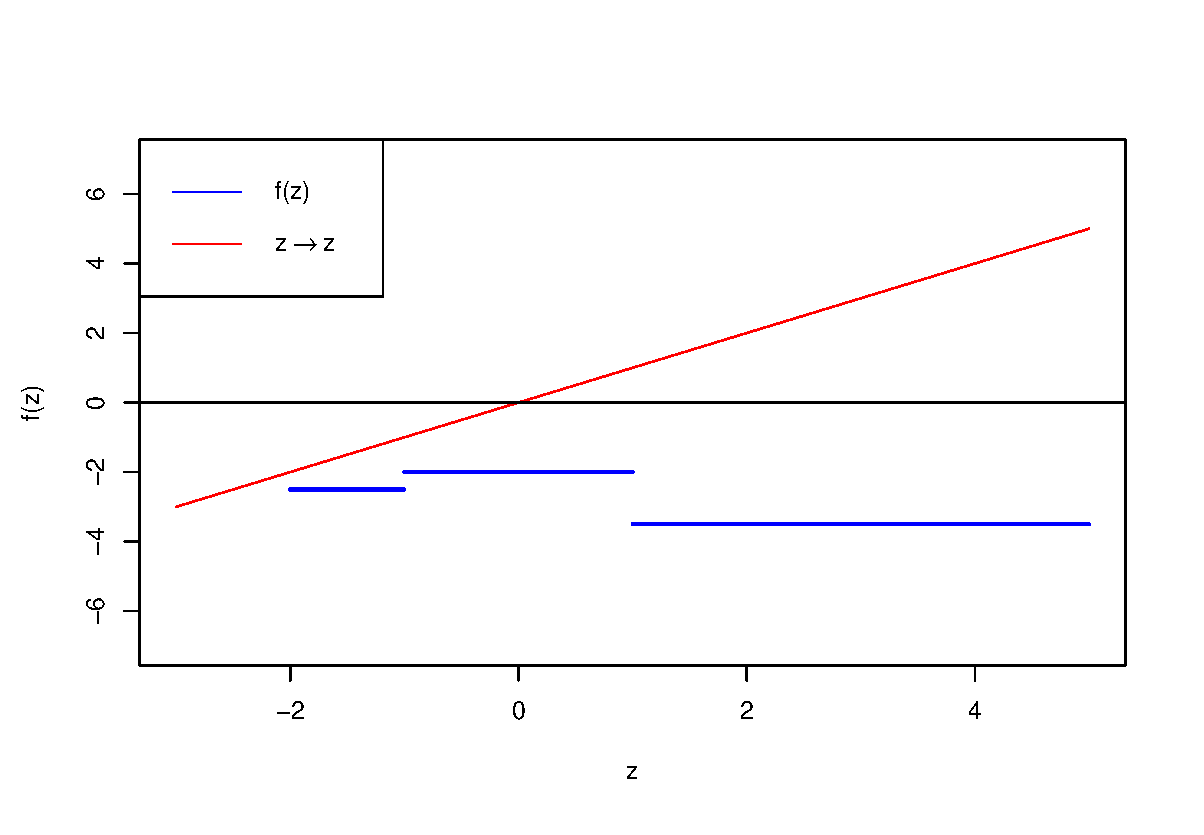
\includegraphics[scale=.5]{Clarke_Plot.eps}
\end{centering}
\end{frame}
\begin{frame}{Existence Counter-Example}
\begin{centering}
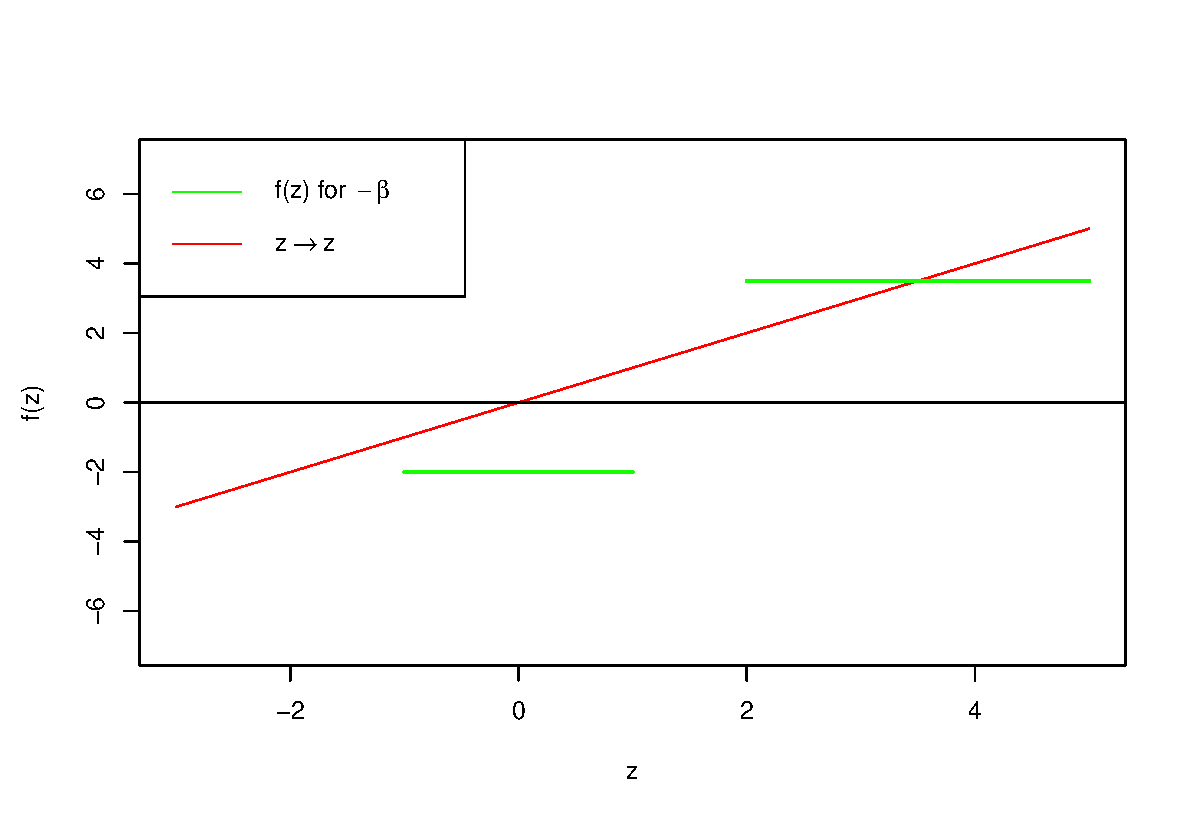
\includegraphics[scale=.5]{Clarke_Plot2.eps}
\end{centering}
\end{frame}

\begin{frame}{One Factor Model with Long Only Constraints (cont.)}
Reformulated Clarke Map.  First, assume without loss of generality $\be^\T \gb>0$.  Define $\psi: \bbr_+  \mapsto \bbr$:
\begin{equation}\label{psieq}
\psi(z) = \frac{\sum_{\{i:z\gb_i<1\}} \gb_i/\gd^2}{1/\gs^2+ \sum_{ \{i:z\gb_i<1\} } \gb_i^2/\gd^2}
\end{equation}
\begin{itemize}
\item This is the reciprocal of $\psi_C$ with a slightly different summand condition.
\item We wish to find $\theta$ such that $\psi(\theta) = \theta$.  
\item$\psi(\cdot)$ is still a discontinuous step function; difficult to work with.
\end{itemize}
\end{frame}


\begin{frame}{One Factor Model with Long Only Constraints (cont.)}
\begin{lemma} Assume $\psi(0)>0$ (equiv. $\be^\T \gb>0$).  Define the function $\phi: \bbr_+ \mapsto \bbr$:
\begin{equation}\label{phi}
\phi(z) = -\gs^2\paren{ \sum_{\{i:z\gb_i<1\}} \frac{\gb_i}{\gd^2}\paren{z \gb_i-1}}.
\end{equation}
A fixed point $\phi(\theta) = \theta$ exists if and only if a fixed point of $\psi(\theta) = \theta$ exists; furthermore, the solutions have the same value.
\end{lemma}
\end{frame}

\begin{frame}{One Factor Model with Long Only Constraints (cont.)}
\begin{lemma}
For $\phi:\bbr_+ \mapsto \bbr$ as defined in Equation \req{phi}, we have the following:
\begin{enumerate}
\item $\phi(z)$ is continuous
\item $\phi(0)>0$
\item $\phi$ is differentiable a.e. and $\phi'(z)<0$ for all $z>0$
\item $\phi(z)$ has a positive root.
\end{enumerate}
\end{lemma}
\end{frame}




\begin{frame}{One Factor Model with Long Only Constraints (cont.)}
\begin{centering}
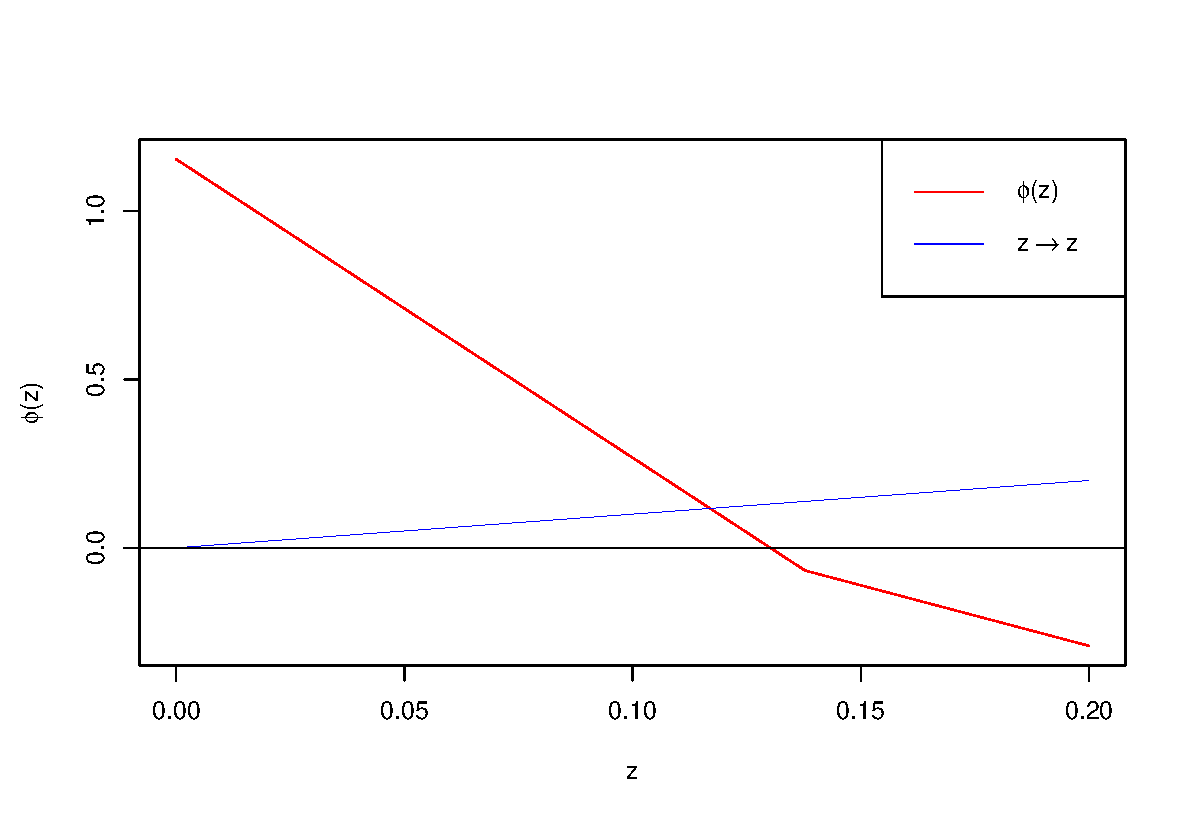
\includegraphics[scale=.5]{FP.eps}
\end{centering}
\end{frame}



\begin{frame}{One Factor Model with Long Only Constraints (cont.)}
\begin{theorem}
There exists a unique nonzero $\theta$ that solves $\phi(\theta)=\theta$
\end{theorem}
This solution is equivalent to the solution to Equation \req{psieq}.
\begin{proof}
This is a straightforward consequence of the Brouwer Fixed-Point Theorem, as  $\phi(\cdot)$ is continuous, $\phi(0)>0$ and for some $z>0$, $\phi(z)=0$.
\end{proof}
\end{frame}

\begin{frame}{Algorithm for One-Factor Model}
Goal: Compute the fixed-point in Equation \req{psieq} under the assumption that $\be^\T \gb/\gd^2 >0$ and $\theta>0$.\\
\textit{Note:} For $\theta$ large enough, $\psi(\theta)$ decreasing and the condition $\theta \gb_i<1$ ensures that every negative $\gb_i$ will be included in the summation.
\begin{itemize}
\item Order $\gb$ vector in increasing order.
\item Starting from $k=p$, compute 
\begin{equation}
\psi_k = \frac{\sum_{i=1}^k\gb_i/\gd^2}{1/\gs^2 \sum_{i=1}^k \gb_i^2/\gd^2}
\end{equation}
\item If $\psi_k \gb_k < 1$, stop, otherwise repeat for $k=k-1$.
\end{itemize}
\end{frame}



\section{Extension to q-Factors}

\begin{frame}{q-Factor Algorithm Setup}
We know that the $\theta$ fixed point solves
\begin{equation}
\theta = \psi(\theta) =\bV \bB^\T \Gd^{-1} \paren{\be - \bB \theta}_+
\end{equation}
However, $\psi(z)$ is not a contraction mapping near the fixed point $\theta$, so we cannot compute fixed point iterations from this formula.

\end{frame}


\begin{frame}{q-Factor Algorithm Setup (cont.)}
Construct the system:
\begin{equation}
\mat{c}_\vartheta = \Gd^{-1}\chi_{\{\be - B \vartheta>0\}}
\end{equation}
\begin{equation}
\mat{b}_\vartheta = \bB^\T \mat{c}_\vartheta
\end{equation}
\begin{equation}
\mat{A}_\vartheta = \bV^{-1} + \bB^\T\mat{diag}(\mat{c}_\vartheta)\bB
\end{equation}
The mapping $\psi(\vartheta) = \mat{A}_\vartheta^{-1} \mat{b}_\vartheta$
defines a q-dimensional mapping equivalent to Equation \req{psieq}.
\end{frame}

\begin{frame}{Fixed Point Algorithm}
We solve the following fixed point:
\[
\begin{aligned}
\Gth &= \gp(\Gth)\\
\Gth &= A_\Gth^{-1} b_\Gth
\end{aligned}
\]
This can be computed as follows:
\begin{enumerate}
\item Initialize $\Gth^0$ as some initial condition; Define $\geps$ as some small tolerance.
\item Iterate $\Gth^{n+1} = A_{\Gth^n}^{-1} b_{\Gth^n}$\\ (or equivalently, solve $A_{\Gth^n}\Gth^{n+1} = b_{\Gth^n}$)
\item Terminate when $\abs{\Gth^{n+1}-\Gth^{n}}<\geps$.
\end{enumerate}
Caveats: This is not guaranteed to converge, as the mapping $\psi(\vartheta)$ is not continuous in $\vartheta$.
\end{frame}

\section{Case Studies}
\begin{frame}{Case Study: Sensitivity with Respect to Factor Variance}
For a fixed $\theta$, we can examine the following partial derivatives:
\begin{equation}
\diff {\gs^2} w_i  = -\frac{\gb_i}{\gd_i^2}\frac{\partial \theta}{\partial \gs^2}
\end{equation}
\begin{equation}
\diff {\gs^2} \theta  = \frac{(\phi(\theta)/\gs^2)}{1 + \gs^2 \sum_{\{i:\theta \gb_i <1 \}} \gb_i^2/\gd_i^2}
\end{equation}
\begin{equation}
\diff {\gs^2} w_i  = \frac{\gb_i \sum_{\{k: \theta \gb_k<1\}} (\gb_k/\gd_k^2)(\theta \gb_k-1)}{\gd_i^2 + \gd_i^2 \gs^2 \sum_{\{k:\theta \gb_k <1 \}} \gb_k^2/\gd_k^2}
\end{equation}
These are ugly formulae...
\end{frame}

\begin{frame}{Derivative of $w_i$ with Respect to $\gs^2$}
\begin{centering}
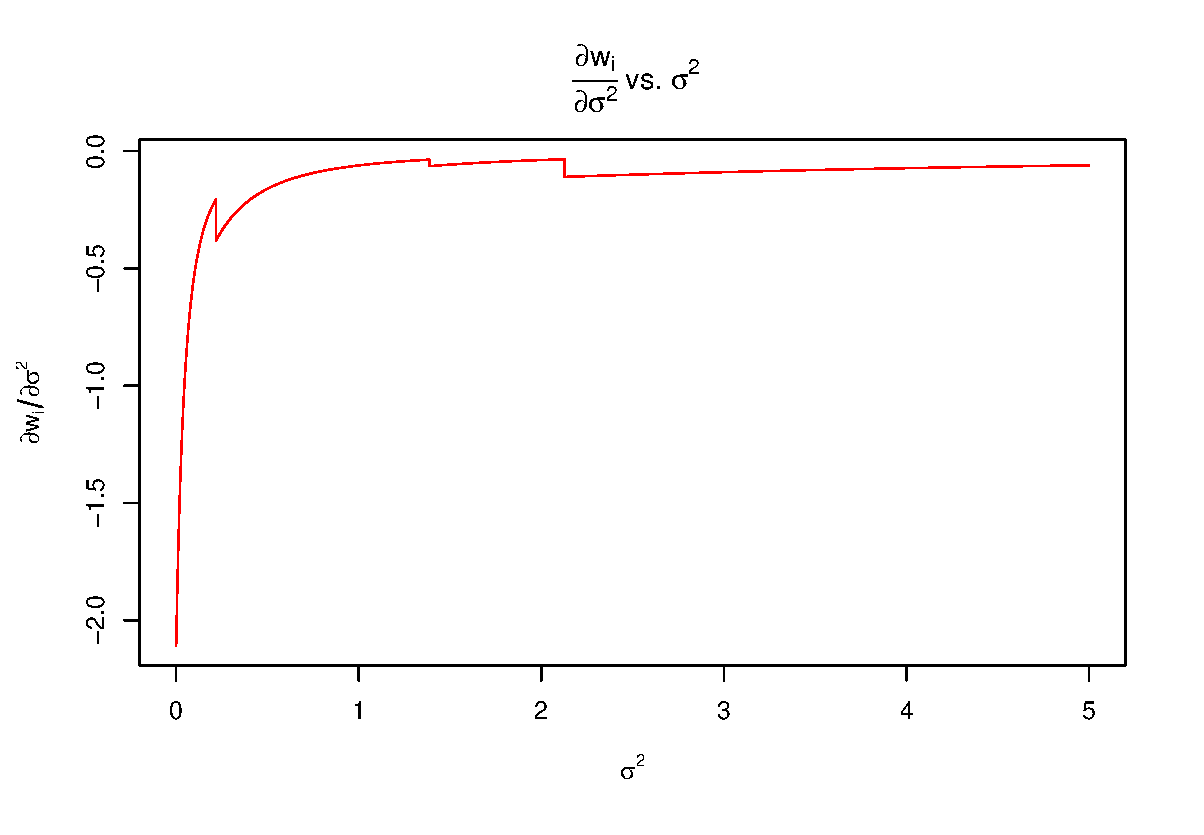
\includegraphics[scale=.5]{sigma_deriva.eps}
\end{centering}
$p=5$, $\gb \sim \ncal_5(1,1)$, $\gd_i^2\sim \mrm{lognorm}(0,1)$.
\end{frame}


\begin{frame}{Derivative of $w_i$ with Respect to $\gs^2$}
\begin{centering}
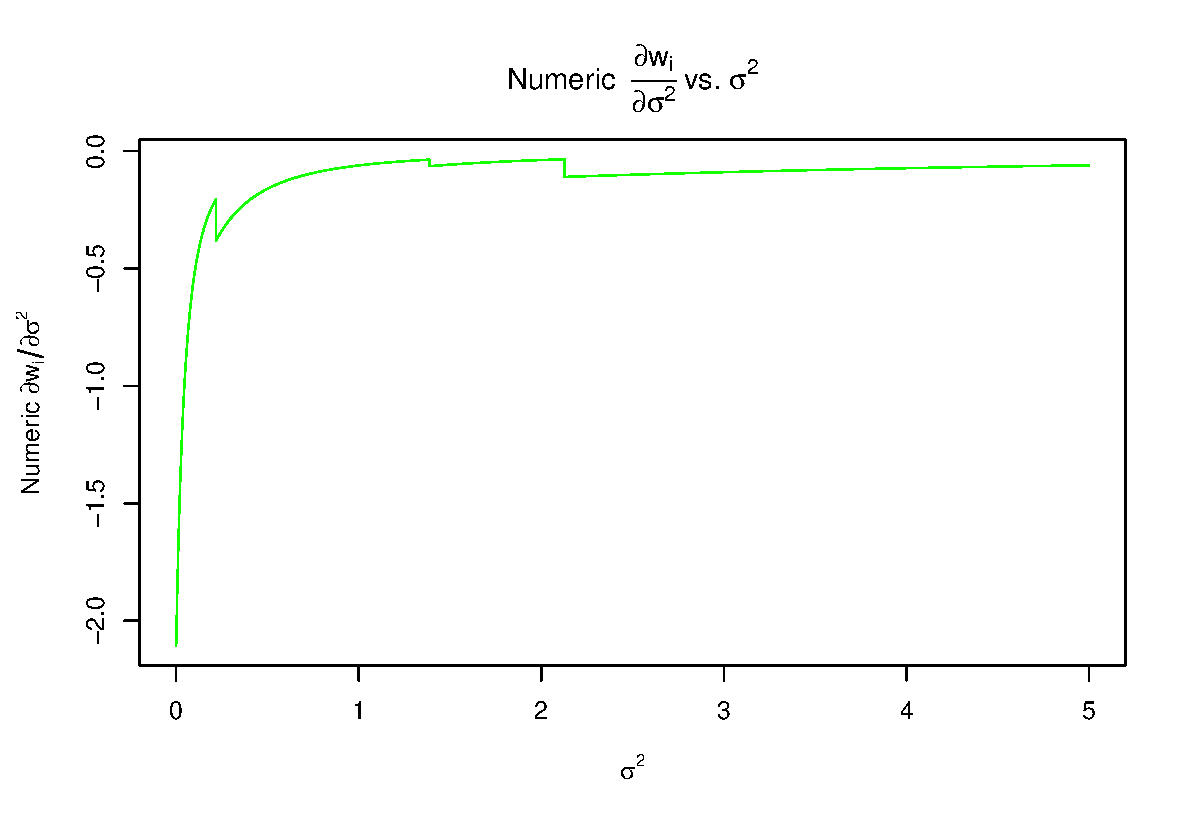
\includegraphics[scale=.5]{sigma_deriva_numeric.eps}
\end{centering}
$p=5$, $\gb \sim \ncal_5(1,1)$, $\gd_i^2\sim \mrm{lognorm}(0,1)$.
\end{frame}

\section{Future Work}



\begin{frame}[allowframebreaks]{References}
\bibliography{siambib}
\bibliographystyle{jmr}

\end{frame}

\end{document}

